\begin{enumerate}[label=\thesection.\arabic*.,ref=\thesection.\theenumi]
\numberwithin{equation}{enumi}

\item
In the Feedback System given below 
\begin{align}
\label{eq:ee18btech11035_G(s)}
 G(s)=\frac{1}{s^2+2s}
\end{align}
The step response of the closed-loop system should have minimum settling time and have no overshoot\\

\begin{figure}[!ht]
    \begin{center}
		
		\resizebox{\columnwidth}{!}{\tikzset{
        block/.style = {draw, rectangle,
            minimum height=1cm,
            minimum width=2cm},
        input/.style = {coordinate,node distance=1cm},
        output/.style = {coordinate,node distance=4cm},
        arrow/.style={draw, -latex,node distance=2cm},
        pinstyle/.style = {pin edge={latex-, black,node distance=2cm}},
        sum/.style = {draw, circle, node distance=1cm},
}

\begin{tikzpicture}[node distance=2.5cm,auto,>=latex']
  \node [input, name=input] {};
  \node [sum, right of=input] (sum) {};
  \node [block, right of = sum] (block1) {$k$};
  \node [block, right of = block1] (block2) {$G(s)$};
  \node [output, right of= block2] (output) {};
  \draw [->] (input) -- node {$r$} (sum);
  \draw [->] (sum) -- node {} (block1);
  \draw [->] (block1) -- node {} (block2);
  \draw [->] (block2) -- node [name =y] {$y$} (output);
  \draw [->] (y) -- ++ (0,-2) -| node [pos=0.99] {$-$} (sum);
\end{tikzpicture}}
	\end{center}
\caption{Block Diagram of given question}
\label{fig:block2}
\end{figure}

\item The required value of gain 'k' to achieve this is\\
\solution Calculating the transfer function of the system\\
\begin{align}
H(s) = \frac{kG(s)}{1+kG(s)}
\label{eq:4}
\end{align}

From \eqref{eq:ee18btech11035_G(s)} Substituting G(s) in \eqref{eq:4} \\
\\Transfer Function becomes 
\begin{align}
H(s) = \frac{k*\frac{1}{s^2+2s}}{1+k*\frac{1}{s^2+2s}}
\end{align}
On further simplifying we get,\\
\begin{align}
H(s) = \frac{k}{s^2+2s+k}
\label{eq:H(s)}
\end{align}\\

For the output to have minimum settling time and also doesn't have overshoot,the system function should also have minimum settling time and also doesn't have overshoot.\\
\\
From \eqref{fig:ee18btech11012}\\
Now, observing the Transfer function of different types systems in time domain. The system which has minimum settling time and also doesn't overshoot is critical damped system.\\
\\
So,when unit step is given as input for critical damped system the output of the system has minimum settling time also the output doesn't overshoot.\\
\\
From \eqref{table:ee18btech11012}\\
Damping ratio(\(\zeta \)) of a critical damped system is 1\\
\\
By comparing the obtained transfer function \eqref{eq:H(s)} with general transfer function of a second order system \eqref{eq:ee18btech11012_second}\\
We get,

\begin{align}
\label{eq:omega}
\omega_n^2 = k,\omega_n = \sqrt{k}\\
\label{eq:zetaomega}
2\zeta\omega_ns = 2s,\zeta\omega_n = 1
\end{align}

From \eqref{eq:omega} and \eqref{eq:zetaomega} \\
\begin{align}
\zeta\sqrt{k} = 1
\label{eq:zetarootk}
\end{align}

As \(\zeta\) = 1  eq\eqref{eq:zetarootk} becomes 
\begin{align}
\sqrt{k} = 1,k = 1
\end{align}

Therefore, Transfer function is 
\begin{align}
H(s) = \frac{1}{s^2+2s+1} = \frac{1}{(s+1)^2}
\end{align}

\item Calculating the output when input is unit step and Verifying that output doesn't overshoot by plotting the output.\\
\solution 
\begin{align}
X(s) = \frac{1}{s}\\
Y(s) = H(s)*X(s)\\
Y(s) = \frac{1}{(s+1)^2}*\frac{1}{s}
\end{align}
Converting Y(s) into partial fraction\\
We get,
\begin{align}
Y(s) = \frac{1}{s}-\frac{1}{s+1}-\frac{1}{(s+1)^2}
\label{Y(s)}
\end{align}

Calculating y(t) by applying the inverse laplace transform for equation \eqref{Y(s)}
\begin{align}
y(t) = (1-e^{-t}-te^{-t})u(t)
\end{align}
Plot of y(t):
\begin{figure}[!h]
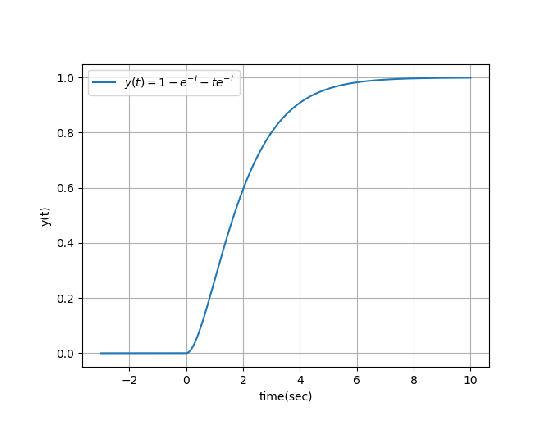
\includegraphics[width=\columnwidth]{./figures/ee18btech11035_3.eps}
\caption{Plot of y(t)}
\label{fig:ee18btech11035_y(t)}
\end{figure}

Python code for the plot y(t) is
\begin{lstlisting}
codes/ee18btech11035_3.py
\end{lstlisting}

The above plot justifies that unit step response doesn't overshoot.

\end{enumerate}
